\chapter{Implementácia}

V tejto kapitole sa budeme zaoberať implementáciou nášho riešenia. Popíšeme si dôvody pre výber jazyka a knižníc a niektoré časti nášho zarovnávača slúžiace na predspracovanie dát, klasifikáciu a zarovnávanie. Potom si popíšeme dôležité pomocné programy -- simulátor a program na trénovanie modelov -- a nakoniec si popíšeme použitie, konfiguráciu a možnosti rozšírenia programu.

\section{Výber jazyka a použité knižnice}
%daky pokec o~tom ze som to pisal v~pythone a preco je python super
Ako jazyk pre písanie nášho zarovnávača sme si vybrali Python (vo verzii 2.7). Dôvodov sme mali niekoľko: V prvom rade zarovnávač sme nepísali od začiatku, ale ako základ sme zobrali zarovnávač od Michala Nánásiho (viď sekcia \ref{subsec:realigner}), ktorý už bol napísaný v jazyku Python 2.7. Ďalšími dôvodmi sú pohodlnosť písania v jazyku Python a dostupnosť veľkého množstva užitočných knižníc. Knižnice pre Python sa dajú písať aj v jazyku C alebo C++, čo umožňuje skĺbiť rýchlosť C a jednoduchosť jazyka Python.

\subsection{Realigner}
\label{subsec:realigner}

\textit{Realigner} je program na zarovnávanie a prezarovnávanie\footnote{modifikáciu existujúceho zarovnania}, ktorý napísal Michal Nánási pre potreby \cite{nanasi2013probabilistic}. Umožňuje prezarovnanie sekvencií pomocou párových HMM a Viterbiho algoritmu. Prezarovnanie dokáže robiť aj v rámci lokálneho okolia okolo pôvodného zarovnania. Program je rozšíriteľný o nové modely, čo sme využili pre naše potreby.

\subsection{Pythonové knižnice}
%  python kniznice - najma scikit-learn, numpy, track
V našom programe sme sa okrem štandardnej knižnice jazyka Python rozhodli využiť niekoľko knižníc. Najdôležitejšími boli knižnice \textit{numpy}, \textit{scipy}, \textit{scikit-learn}, \textit{pyplot}, \textit{track} a \textit{pandas}.

Numpy je matematická knižnica, ktorá obsahuje množstvo užitočných matematických funkcií. Pre nás z nej boli dôležité hlavne štatistické funkcie, napr. generovanie náhodných čísel z rôznych rozdelení a počítanie štandardnej odchýlky. Okrem toho je táto knižnica základom aj pre väčšinu ostatných použitých knižníc.

Scipy obsahuje funkcie pre pokročilejšie vedecké výpočty. My sme z nej využili hlavne funkciu na odhad rozdelenia pomocou gausiánov.

Scikit-learn je knižnica zaoberajúca sa hlavne strojovým učením. Odtiaľ sme využili náhodné lesy.

Pyplot je knižnica na kreslenie grafov a využili sme ju na vygenerovanie všetkých našich vizualizácií.

Track je knižnica na prácu s {\tt '.bed'} súbormi, v ktorých sme mali uložené naše anotácie.

Pandas je knižnica na analýzu a úpravu veľkých dát. Poslúžila nám najmä pri príprave anotácií pre biologické zarovnania.

\section[Triedy na zarovnávanie s klas.]{Triedy na zarovnávanie s~klasifikátorom}

V tejto sekcii si popíšeme najdôležitejšie triedy, ktoré sme doplnili do programu Realigner. Ide o triedy na presdpracovanie dát, klasifikáciu a triedy pre stavy pHMM.

\subsection{Predspracovanie dát}

\todo obrazok classdiagramu

Na predspracovanie dát nám slúžili triedy \textit{DataPreparer}, \textit{ComparingDataPreparer}, \textit{FullComparingDataPreparer}, \textit{CombinedDataPreparer},
\textit{IndelDataPreparer}, \textit{ComparingIndelDataPreparer}, \textit{FullComparingIndelDataPreparer} a \textit{CombinedIndelDataPreparer} (obr \ref{fig:classdiagram-preparers}).

Trieda DataPreparer je rodičovskou triedou pre ostatné triedy, takže si popíšeme najmä ju. Trieda IndelDataPreparer je rodičom Indel verzií tried. Tieto triedy majú dve hlavné úlohy: Prvá je predpríprava dát na klasifikáciu a druhá je výroba trénovacej množiny zo sekvencií.

Pri predpríprave dát je úlohou dať dáta do formy vhodnej pre klasifikátor. To znamená získať okno a anotácie a ďalšie atribúty tak ako sme ich popísali v kapitole \ref{subsec:attribute-selection} a previesť ich do číselnej podoby. Naše štyri typy tried, ktoré zodpovedajú štyrom typom dát, sa líšia iba v tejto úlohe. Najdôležitejšia práca sa vykoná v metóde \method{\_prepare\_sequence}, ktorá pripraví dáta pre jednu sekvenciu, a potom sa zlepia dáta z volania tejto funkcie pre obe sekvencie. Indel verzie tried obsahujú príslušné úpravy aby v sekvencii s medzerou použili kratšie okno.

Pri predspracovaní trénovacej množiny treba zo zarovnaní vytvoriť pozitívne a negatívne príklady. Táto metóda je implementovaná len v DataPreparer a IndelDataPreparer triede, ostatné ju zdedia. Pri výbere pozitívnych príkladov v triede DataPreparer označujeme pozície v sekvencii, ktoré sú zarovnané. To má na starosti metóda \method{prepare\_positive\_data}. Metóda \method{prepare\_negative\_data} vyberá negatívne príklady použitím zarovnaných pozícií z pozitívnych príkladov a náhodne ich poposúva podľa vzorca spomenutého v sekcii \ref{subsec:clf-training}. Okrem toho sme implementovali aj náhodný výber negatívnych dát v metóde \method{prepare\_negative\_data\_random}, kde negatívne príklady vyberáme náhodne z nezarovnaných pozícií s tým, že vyberieme rovnako veľa negatívnych ako pozitívnych príkladov. V Indel klasifikátore sa oba typy príkladov vyberajú v metóde \method{prepare\_training\_data}, pričom jedna sekvencia sa zvolí za medzerovú a za pozitívne príklady sa vezme všetko, čo je zarovnané k medzere v medzerovej sekvencii. Za negatívne sa vezme rovnako veľa náhodných zarovnaných pozícií.

\subsection{Abstrakcia klasifikátora}
\label{subsec:pairclassifier}
V pre väčšiu modularitu sme sa rozhodli naprogamovať vrstvu medzi klasifikátorom a zvyškom programu. Trieda sprostredkúvajúca túto vrstvu sa volá \textit{PairClassifier}. PairClassifier poskytuje niekoľko metód navyše oproti tým, ktoré poskytuje klasifikátor.
Jej hlavnými výhodami sú:

\begin{itemize}
    \item možnosť rýchlej výmeny klasifikátora bez úpravy zvyšku programu
    \item automatické predspracovanie pri klasifikácii a trénovaní pomocou príslušnej triedy DataPreparer
    \item automatické trénovanie -- ak klasifikátor nie je natrénovaný, tak sa automaticky natrénuje z prednastavenej trénovacej množiny
    \item hromadná klasifikácia s predspracovaním
    \item otočenie výstupu klasifikátora
\end{itemize}

\subsection{HMM stavy s~klasifikátorom}
\label{subsec:hmm-states}

V zarovnávači bol implementovaný Viterbiho algoritmus, ktorý pracoval s párovými HMM. Tento algoritmus pracoval s triedou \textit{GeneralizedPairState}, ktorá poskytovala metódu \method{emission} vracajúcu emisiu báz na daných pozíciách. Od tejto triedy dedia naše triedy \textit{ClassifierState}, \textit{ClassifierIndelState}, ktoré tvoria náš model~A a preťažili sme metódu \method{emission} tak, aby vracala hodnoty z klasifikátora. Museli sme však urobiť niekoľko zmien. Viterbiho algoritmus si pýta emisie po jednej. Avšak volanie C-čkovej funkcie z knižnice scikit-learn z Pythonu je pomalé, takže pre dlhé sekvencie by zarovnanie trvalo veľmi dlho. Preto sme si najskôr naraz, počas jedného volania funkcie predpočítali emisie pre všetky pozície a tie sme potom zapamätali a vracali v momente, keď si ich Viterbiho algoritmus vypýtal. Na to sme využili možnosť hromadnej klasifikácie v našej triede PairClassifier (sekcie \ref{subsec:pairclassifier}). Tieto dve triedy sa líšia iba v použitej triede na predspracovanie dát.

Od tried ClassifierState a ClassifierIndelState potom dedia triedy \textit{ClassifierAnnotationState} a \textit{ClassifierAnnotationIndelState}, ktoré tvoria diskrétnu verziu nášho modelu~B. Triedy mali v súbore uložené tabuľky emisií a podľa aktuálnych pozícií si zistili bázy a aktuálny výstup klasifikátora, ktoré slúžili ako indexy do tabuľky. Tieto triedy navyše obsahujú metódy na trénovanie emisií.

Od ClassifierAnnotationState a ClassifierAnnotationIndelState dedia triedy \textit{ContignuousClassifierAnnotationState} a \textit{ContignuousClassifierAnnotationIndelState}, ktoré stvárňujú spojitú verziu modelu~B. Tieto triedy majú v tabuľke emisií pre každú dvojicu báz uloženú serializovanú verziu objektu \textit{gaussian\_kde} (viac detailov je v sekcii \ref{subsec:impl-model-traioning}), ktorý obsahuje distribúciu výstupu klasifikátora. Konkrétnu hodnotu potom získa volaním príslušného objektu k danej dvojici báz (resp. báze pri IndelState) s hodnotou klasifikátora. Tieto triedy takisto obsahujú aj metódy na trénovanie emisií.

Od triedy \textit{GeneralizedPairState} navyše dedia aj naše triedy pre referenčný model -- \textit{SimpleMatchState} a \textit{SimpleIndelState}, ktoré triedu GeneralizedPairState rozširujú o metódy na trénovanie emisných pravdepodobností.

\todo obrazok classdiagramu

\section{Pomocné programy}
V tejto sekcii sa budeme venovať dvom hlavným pomocným programom. Prvým z nich je náš simulátor, ktorý nám umožňuje generovať zarovnania a druhým je program na trénovanie zarovnaní. Okrem toho sme implementovali množstvo programov na tvorbu vizualizácií pre túto prácu, alebo konverziu dát z rôznych zdrojov do formátov podporovaných našim zarovnávačom, o ktorých si však hovoriť nebudeme.
\subsection{Simulátor}
\label{subsec:simulator}

Simulátor slúži na generovanie zarovnaní pre naše experimenty. Náhodne vygeneruje tri\footnote{aby sme vedeli počítať tranzitivitu} sekvencie, ktoré vznikli zo spoločného predka a vyrobí korektné spoločné zarovnanie všetkých troch sekvencií. Okrem toho vyrobí aj dodatočné informácie, ktoré majú pomôcť pri zarovnávaní.

\subsubsection{Algoritmus}
Ako prvú simulátor vygeneruje informáciu o~tom, ktoré časti sekvencie prislúchajú génom a ktoré nie. Informácia má podobu binárneho vektora.
Najskôr sa informácia vygeneruje pre \textit{základnú (master) sekvenciu} a z nej sa potom skopíruje do troch dcérskych sekvencií, pričom s určitou pravdepodobnosťou sa niektoré gény zmažú (jednotky sa prepíšu na nulu). Táto informácia bude tvoriť pásku s anotáciou o géne.

Potom simulátor vygeneruje základnú sekvenciu a z~nej následne pomocou mutácie a delécie (inzercia = delécia v zvyšných sekvenciách) odvodí tri ďalšie sekvencie. Mutácia má rôzne pravdepodobnosti v prípade, že ide o gén v jednej či druhej sekvencii, alebo oboch.
Simulátor rovno generuje zarovnanie tým, že keď robí deléciu, nahradzuje bázy pomlčkami.

% Simulátor má vopred daných niekoľko konštánt -- pravdepodobnosti udalostí, ktoré môžu nastať.

\subsubsection{Generovanie informácie o~génoch}
% Ak sa na danom mieste nachádza gén, označíme to $1$ inak $0$.
\todo awk:
Gény bývajú súvislé úseky, takže ich treba generovať tak, že niekedy začneme gén, potom generujeme jednotky, potom skončíme gén a generujeme nuly. Potom môžme opäť začať gén atď.

\begin{figure}[htp]
    \centering
    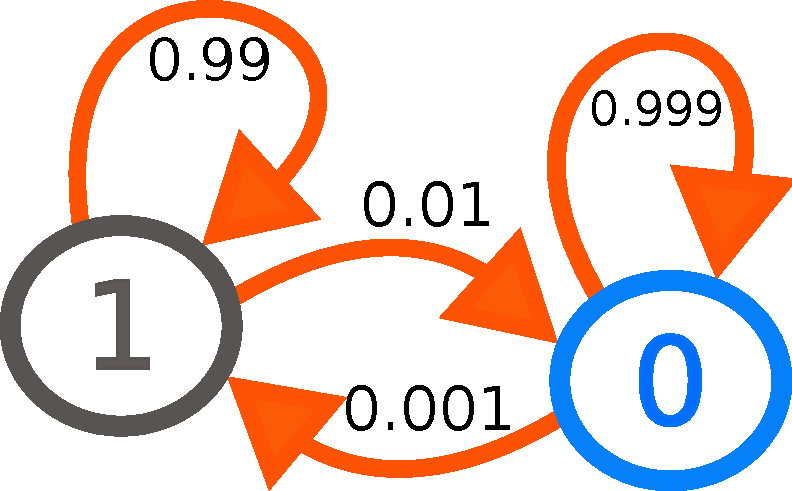
\includegraphics[width=.7\textwidth]{images/markov_chain}
    \caption[Markovova reťaz použitá na generovanie informácie o~génoch]{Markovova reťaz použitá na generovanie informácie o~génoch. $p$ je pravdepodobnosť, že začneme generovať gén, $q$ je pravdepodobnosť, že prestaneme generovať gén.}
    \label{fig:markov-chain}
\end{figure}

Generovanie robíme pomocou \textit{Markovovskej reťaze (Markov Chain)} obr. \ref{fig:markov-chain}. Generujeme podľa aktuálneho stavu a v~každom kroku sa náhodne rozhodneme, či sa prepneme do iného stavu, alebo ostaneme v~tom istom. Rozhodnutie robíme pomocou \textit{falošnej mince (biased coin)}, kde hlava padne s danou pravdepodobnosťou, ktorú nastavíme ako parameter. V našom prípade je to $p$ pre stav nula a $q$ pre stav jedna.

%TODO ak bude treba zabrat miesto, tak sem drbnut nejake zdrojaky

\subsubsection{Simulácia mutácie a delécie}

Ak už máme vygenerovanú základnú sekvenciu, potom vyrobíme zmutovanú sekvenciu tak, že s~určitou pravdepodobnosťou nahradíme bázu zo~základnej sekvencie inou bázou. Pravdepodobnosť závisí aj od toho, či je na danej pozícii gén v~oboch sekvenciách, v~jednej, alebo v~žiadnej. Na rozhodovanie máme pre každú možnosť jednu falošnú mincu a podľa toho, ktorá z~možností nastala, hodíme si príslušnou mincou.

Deléciu simulujeme opäť pomocou podobnej Markovovskej reťaze, pretože počas evolúcie majú tendenciu vypadávať súvislé úseky. Stav nula bude, že nemažeme a stav jedna, že mažeme, teda nahradzujeme danú bázu znakom {\verb+'-'+}.

\subsubsection{Využitie}

Simulátor je prvá vec, ktorú sme implementovali a slúžil na väčšinu našich experimentov. Simulované dáta majú totiž oproti biologickým niekoľko výhod. Prvou je, že poznáme správnu odpoveď, a teda môžme objektívne zhodnotiť úspešnosť našich modelov. Druhou je možnosť zvoliť si parametre, ktoré menia závislosť mutácií na anotáciách a testovať správanie modelov, ak zvýšime túto závislosť. Ďalšou výhodou je, že si môžme vygenerovať ľubovoľne veľa ľubovoľne dlhých sekvencií.

\subsection{Trénovanie modelov}
\label{subsec:impl-model-traioning}

Trénovanie modelov má na starosti trieda \textit{ModelTraining} a je urobené pomocou metódy maximálnej vierohodnosti (kapitola \ref{subsec:hmmtraining}).
Trénovanie prechodových pravdepodobností je pre všetky modely spoločné. Trénovanie emisných pravdepodobností je v každom stave spravené zvlášť, pretože stavy emitujú rôzne symboly a jednotlivé stavy majú rôzne spôsoby trénovania.
Trieda ModelTraining najskôr načíta model z ktorého zistí stavy.
Potom načíta trénovacie sekvencie a oanotuje ich stavmi. Následne vypočíta prechodové pravdepodobnosti. Spočíta všetky výskyty nasledujúcich stavov vo všetkých sekvenciách pre každý stav zvlášť. To vydelí celkovým počtom výskytov daného stavu. Potom oanotované sekvencie predloží jednotlivým stavom, aby vypočítali emisné pravdepodobnosti.

Máme štyri základné typy stavov, ktoré sme si popísali v časti \ref{subsec:hmm-states} a pre každý máme triedu pre Match a Inzert verziu:
\begin{itemize}
    \item SimpleMatchState, SimpleIndelState
    \item ClassifierState, ClassifierIndelState
    \item ClassifierAnnotationState, ClassifierAnnotationIndelState
    \item ContignuousClassifierAnnotationState, ContignuousClassifierAnnotationIndelState
\end{itemize}

V SimpleMatchState, SimpleIndelState algoritmus priamo spočíta výskyty príslušných dvojíc báz (resp. báz) a vydelí celkovým počtom výskytu stavu.
V ClassifierState, ClassifierIndelState sa emisie netrénujú, takže tabuľka bude prázdna.
V ClassifierAnnotationState, ClassifierAnnotationIndelState sa pre každý stav a pre každú dvojicu báz (resp. bázu) spočítajú hodnoty z klasifikátora a tie sa následne aproximujú pomocou gausiánov. Na toto využijeme triedu \method{gaussian\_kde} z modulu \method{scipy.stats}. Táto trieda robí odhad distribučnej funkcie z množiny hodnôt. Šírku pásma (parameter, ktorý určuje hladkosť výslednej funkcie) sme nechali na predvolenej hodnote -- ,,scott''. Tá nastavuje šírku pásma podľa vzorca:
$$n^{-1/(d+4)},$$
kde $n$ je počet vstupov a $d$ je počet dimenzií (v našom prípade $d = 1$). Viac detailov je v \cite{scipydoc} alebo \cite{wiki:kde}. Následne túto funkciu diskretizujeme na $k$ hodnôt. To spravíme pomocou určitého integrálu, pomocou metódy \method{integrate\_box(a, b)}, ktorá spočíta určitý integrál od $a$ po $b$.
Keďže gaussian\_kde je definovaný na intervale $\left<-\infty, \infty \right>$ a $$\int_{-\infty}^\infty \! gaussian\_kde(x) \mathrm{d}x = 1,$$ orezaním definičného oboru na $\left<0,1\right>$ sa môže stať, že $$\int_0^1 \! gaussian\_kde(x) \mathrm{d}x < 1.$$ V tom prípade výslednú hodnotu ešte musíme normalizovať vydelením hodnotou $$\mu = \int_0^1 \! gaussian\_kde(x) \mathrm{d}x.$$ Ako sme si ukázali v \ref{sec:model-training} výslednú pravdepodobnosť dopočítame vynásobením diskretizovanej pravdepodobnosti daného výstupu klasifikátora v prípade daných báz a pravdepodobnosti daných báz.
V ContignuousClassifierAnnotationState, ContignuousClassifierAnnotationIndelState postupujeme rovnako, ako v predchádzajúcom prípade, ale distribúciu už nediskretizujeme. Namiesto toho si ju uložíme do súboru ako $g$ spolu s číslom $\lambda = p/\mu$, kde $p$ je pravdepodobnosť daných báz a $\mu$ je normalizačná konštanta -- tá istá ako v predchádzajúcom prípade. Hustotu emisie potom počas zarovnávania vypočítame tak, že zoberieme parametre pre danú dvojicu báz (resp. bázu) -- $g$ a $\lambda$ -- a pre výstup klasifikátora $c$ bude hustota $f(c) = \lambda g(c).$
% \subsection{Testovanie klasifikátora}
% \todo random\_forest\_evaluation.py

\section{Použitie}

Hlavný program sa spúšťa príkazom
\begin{verbatim}
    PYHONPATH=. python bin/Realigner.py vstup výstup
\end{verbatim}
s následujúcimi parametrami
\begin{itemize}
    \item \method{--mathtype}: float/LogNum -- označuje, či sa má počítať s logaritmovanými hodnotami alebo s reálnymi
    \item \method{--algorithm}: viterbi -- v našich modeloch je podporovaný len viterbi
    \item \method{--beam\_width}: číslo -- šírka okolo lúča vstupného zarovnania, ktorá sa má prehľadávať vo viterbiho algoritme
    \item \method{--model}: ClassificationHMM.js/OracleHMM.js/SimpleHMM2.js/vlastný -- model, ktorý sa má použiť (naše modely sa nachádzajú v data/models)
    \item \method{--sequence\_regexp}: sekvenciaX sekvenciaY regulárne výrazy na vyfiltrovanie dvoch sekvencií zo vstupného súboru zarovnania
    \item \method{--annotation\_model}: súbor.js -- súbor s konfiguráciou anotácií pre jednotlivé sekvencie
\end{itemize}
Pozičné parametre
\begin{itemize}
    \item \method{1}: vstup -- súbor so vstupným zarovnaním
    \item \method{2}: výstup -- súbor kam sa má uložiť výstupné zarovnanie
\end{itemize}
Napríklad:
\begin{verbatim}
    PYHONPATH=. python bin/Realigner.py\
         --mathType LogNum --algorithm viterbi --beam_width 30\
         --model data/models/ClassificationHMM.js\
         --sequence_regexp ^sequence1$ ^sequence2$\
         --annotation_model annotations.js\
         input_alignment.fa output_alignment.fa
\end{verbatim}

Predtým, ako prvýkrát spustíme zarovnávač, je nutné model najskôr natrénovať. To spravíme spustením programu
\begin{verbatim}
python model_training.py  model trénovacie_dáta,
\end{verbatim}
kde prvý parameter je model, ktorý chceme trénovať a druhý je adresár s trénovacími sekvenciami. Ak ešte nemáme natrénovaný klasifikátor, tak sa natrénuje automaticky z dát ktoré sa nachádzajú v priečinku {\tt data/sequences/train\_sequences}. Napríklad
\begin{verbatim}
python model_training.py\
    data/models/OracleHMM.js data/sequences/model_training/bio,
\end{verbatim}

Klasifikátor sa potom uloží do {\tt data/clf} odkiaľ sa bude automaticky načítavať aj pri trénovaní modelov aj pri zarovnávaní. Pokiaľ treba klasifikátor natrénovať odznovu, je nutné ho z {\tt data/clf} vymazať.

\subsection{Konfigurácia a Formáty súborov}
Konfigurácia našich modelov sa nachádza v dvoch súboroch:
\begin{itemize}
    \item {\tt classifier\_alignment/constants.py} -- tu sa dá zmeniť veľkosť okna a či sú povolené anotácie
    \item {\tt classifier\_alignment/config.py} -- tu sa dá zmeniť klasifikátor, datapreparer a  či sa má použiť ten istý klasifikátor aj na Match aj na Inzert stav alebo nie. V tomto súbore sú preddefinované klasifikátory a datapreparer-y takže stačí zmeniť index označujúci, ktorý z nich sa má použiť.
\end{itemize}

Súbory zarovnania sú vo formáte FASTA\footnote{\url{http://en.wikipedia.org/wiki/FASTA_format}}, súbory anotácií sú vo formáte BED\footnote{\url{http://genome.ucsc.edu/FAQ/FAQformat.html\#format1}}.

Súbory modelov sú vo formáte JSON\footnote{JavaScript object notation}, nasledujúceho tvaru:

\begin{lstlisting}
{
  "model": {
    "states": [
      {
        "name": "Match",
        "durations": [[[1, 1], 1.0]],
        "startprob": 0.33,
        "endprob": 1.0,
        "emission": [],
        "onechar": "M",
        "__name__": "SimpleMatchState"
      },
      {
        "name": "InsertX",
        "durations": [[[1, 0], 1.0]],
        "startprob": 0.33,
        "endprob": 1.0,
        "emission": [],
        "onechar": "X",
        "__name__": "SimpleIndelState"
      },
      {
        "name": "InsertY",
        "durations": [[[0, 1], 1.0]],
        "startprob": 0.33,
        "endprob": 1.0,
        "emission": [],
        "onechar": "Y",
        "__name__": "SimpleIndelState"
      }
    ],
    "__name__": "GeneralizedPairHMM",
    "transitions": []
  }
}
\end{lstlisting}

% [["A", "A"], 0.16829558998808106],
% [["A", "T"], 0.026758045292014303],
% [["T", "T"], 0.17806912991656734],
% [["T", "A"], 0.026758045292014303],
% [["G", "G"], 0.17234803337306318],
% [["C", "T"], 0.027234803337306317],
% [["T", "C"], 0.027234803337306317],
% [["G", "A"], 0.02437425506555423],
% [["G", "T"], 0.027234803337306317],
% [["A", "C"], 0.02497020262216925],
% [["A", "G"], 0.02437425506555423],
% [["G", "C"], 0.024493444576877233],
% [["C", "C"], 0.17115613825983314],
% [["T", "G"], 0.027234803337306317],
% [["C", "G"], 0.024493444576877233],
% [["C", "A"], 0.02497020262216925]

% ["A", 0.2526041666666667],
% ["C", 0.23046875],
% ["T", 0.25390625],
% ["G", 0.2630208333333333]

% ["A", 0.2526041666666667],
% ["C", 0.23046875],
% ["T", 0.25390625],
% ["G", 0.2630208333333333]'

Emisné a prechodové tabuľky sa vyplnia pri trénovaní modelu. Zaujímavé sú pre nás len položky \method{\_\_name\_\_} v jednotlivých stavoch. Tam treba vložiť meno príslušnej triedy pre stav.

Súbor pre konfiguráciu anotácií je JSON následujúceho tvaru:
\begin{lstlisting}
{
  "__name__": "Annotations",
  "annotations": ["gene"],
  "sequences": [
    {
      "name": "sequence1", "annotations": [
        {
          "id": "gene",
          "file": "data/sequences/simulated/simulated_alignment_sequence1_gene.bed"
          "offset": 47
        }
      ]
    },
    {
      "name": "sequence2", "annotations": [
        {
          "id": "gene",
          "file": "data/sequences/simulated/simulated_alignment_sequence2_gene.bed"
          "offset": 47
        }
      ]
    },
    {
      "name": "sequence3", "annotations": [
        {
          "id": "gene",
          "file": "data/sequences/simulated/simulated_alignment_sequence3_gene.bed"
          "offset": 47
        }
      ]
    }
  ]
}
\end{lstlisting}
Do \method{annotations} treba dať zoznam anotácií ktoré sa majú použiť a do \method{sequences} treba dať zoznam sekvencií -- meno musí byť rovnaké ako vo FASTA súbore. Pre každú sekvenciu treba vyplniť v \method{annotations} pre každú anotáciu (id musí byť rovnaké ako v zozname anotácií) zdrojový súbor, odkiaľ sa má daná anotácia načítať. Navyše je možné špecifikovať \method{offset} v prípade, že sekvencia, ktorú chceme zarovnať, nezačína v genóme na pozícii 0 a anotácie sú číslované podľa pozícií v genóme.

\section{Rozšírenie programu}

Program je možné ľahko rozšíriť rôznymi spôsobmi. Je možné pridať:
\begin{itemize}
    \item novú triedu pre stav
    \item nový DataPreparer
    \item nový klasifikátor
\end{itemize}

Nová trieda pre stav musí dediť od GeneralizedPairState, alebo niektorého z jej potomkov. Najdôležitejšiou metódou je emission, ktorá dostane dve pozície, dve sekvencie a dve hodnoty, ktoré označujú koľko symbolov z ktorej sekvencie treba vygenerovať, jej výstupom je pravdepodobnosť, že sa vygenerujú dané znaky z daných sekvnecií od daných pozícií. Ak chceme túto triedu použiť v modeli, musíme ju ešte zaregistrovať do triedy \textit{HMMLoader} pomocou metódy \method{addFunction}.

Nový DataPreparer musí dediť od triedy DataPreparer, alebo niektorej z jej potomkov. Najdôležitejšou je metóda \method{prepare\_data}, ktorá dostane obe sekvencie, anotácie a aj dve pozície v sekvenciách. Výstupom musí byť pole číselných atribútov. Preťažením metódy \method{prepare\_training\_data} sa dá zmeniť generovanie trénovacej množiny.

Nový klasifikátor musí implementovať nasledujúce metódy:
\begin{itemize}
    \item \method{fit(X, y)} -- dostane pole trénovacích vektorov a pole cieľových hodnôt, z ktorých natrénuje svoje parametre
    \item \method{predict\_proba(X)} -- dostane pole vstupných vektorov a výstupom je dvojrozmerné pole -- pre každý vstupný vektor a každú triedu pravdepodobnosť, že vektor patrí do danej triedy
\end{itemize}
Navyše musí byť serializovateľný pomocou modulu \textit{pickle}.
